\documentclass[1p]{elsarticle_modified}
%\bibliographystyle{elsarticle-num}

%\usepackage[colorlinks]{hyperref}
%\usepackage{abbrmath_seonhwa} %\Abb, \Ascr, \Acal ,\Abf, \Afrak
\usepackage{amsfonts}
\usepackage{amssymb}
\usepackage{amsmath}
\usepackage{amsthm}
\usepackage{scalefnt}
\usepackage{amsbsy}
\usepackage{kotex}
\usepackage{caption}
\usepackage{subfig}
\usepackage{color}
\usepackage{graphicx}
\usepackage{xcolor} %% white, black, red, green, blue, cyan, magenta, yellow
\usepackage{float}
\usepackage{setspace}
\usepackage{hyperref}

\usepackage{tikz}
\usetikzlibrary{arrows}

\usepackage{multirow}
\usepackage{array} % fixed length table
\usepackage{hhline}

%%%%%%%%%%%%%%%%%%%%%
\makeatletter
\renewcommand*\env@matrix[1][\arraystretch]{%
	\edef\arraystretch{#1}%
	\hskip -\arraycolsep
	\let\@ifnextchar\new@ifnextchar
	\array{*\c@MaxMatrixCols c}}
\makeatother %https://tex.stackexchange.com/questions/14071/how-can-i-increase-the-line-spacing-in-a-matrix
%%%%%%%%%%%%%%%

\usepackage[normalem]{ulem}

\newcommand{\msout}[1]{\ifmmode\text{\sout{\ensuremath{#1}}}\else\sout{#1}\fi}
%SOURCE: \msout is \stkout macro in https://tex.stackexchange.com/questions/20609/strikeout-in-math-mode

\newcommand{\cancel}[1]{
	\ifmmode
	{\color{red}\msout{#1}}
	\else
	{\color{red}\sout{#1}}
	\fi
}

\newcommand{\add}[1]{
	{\color{blue}\uwave{#1}}
}

\newcommand{\replace}[2]{
	\ifmmode
	{\color{red}\msout{#1}}{\color{blue}\uwave{#2}}
	\else
	{\color{red}\sout{#1}}{\color{blue}\uwave{#2}}
	\fi
}

\newcommand{\Sol}{\mathcal{S}} %segment
\newcommand{\D}{D} %diagram
\newcommand{\A}{\mathcal{A}} %arc


%%%%%%%%%%%%%%%%%%%%%%%%%%%%%5 test

\def\sl{\operatorname{\textup{SL}}(2,\Cbb)}
\def\psl{\operatorname{\textup{PSL}}(2,\Cbb)}
\def\quan{\mkern 1mu \triangleright \mkern 1mu}

\theoremstyle{definition}
\newtheorem{thm}{Theorem}[section]
\newtheorem{prop}[thm]{Proposition}
\newtheorem{lem}[thm]{Lemma}
\newtheorem{ques}[thm]{Question}
\newtheorem{cor}[thm]{Corollary}
\newtheorem{defn}[thm]{Definition}
\newtheorem{exam}[thm]{Example}
\newtheorem{rmk}[thm]{Remark}
\newtheorem{alg}[thm]{Algorithm}

\newcommand{\I}{\sqrt{-1}}
\begin{document}

%\begin{frontmatter}
%
%\title{Boundary parabolic representations of knots up to 8 crossings}
%
%%% Group authors per affiliation:
%\author{Yunhi Cho} 
%\address{Department of Mathematics, University of Seoul, Seoul, Korea}
%\ead{yhcho@uos.ac.kr}
%
%
%\author{Seonhwa Kim} %\fnref{s_kim}}
%\address{Center for Geometry and Physics, Institute for Basic Science, Pohang, 37673, Korea}
%\ead{ryeona17@ibs.re.kr}
%
%\author{Hyuk Kim}
%\address{Department of Mathematical Sciences, Seoul National University, Seoul 08826, Korea}
%\ead{hyukkim@snu.ac.kr}
%
%\author{Seokbeom Yoon}
%\address{Department of Mathematical Sciences, Seoul National University, Seoul, 08826,  Korea}
%\ead{sbyoon15@snu.ac.kr}
%
%\begin{abstract}
%We find all boundary parabolic representation of knots up to 8 crossings.
%
%\end{abstract}
%\begin{keyword}
%    \MSC[2010] 57M25 
%\end{keyword}
%
%\end{frontmatter}

%\linenumbers
%\tableofcontents
%
\newcommand\colored[1]{\textcolor{white}{\rule[-0.35ex]{0.8em}{1.4ex}}\kern-0.8em\color{red} #1}%
%\newcommand\colored[1]{\textcolor{white}{ #1}\kern-2.17ex	\textcolor{white}{ #1}\kern-1.81ex	\textcolor{white}{ #1}\kern-2.15ex\color{red}#1	}

{\Large $\underline{12n_{0088}~(K12n_{0088})}$}

\setlength{\tabcolsep}{10pt}
\renewcommand{\arraystretch}{1.6}
\vspace{1cm}\begin{tabular}{m{100pt}>{\centering\arraybackslash}m{274pt}}
\multirow{5}{120pt}{
	\centering
	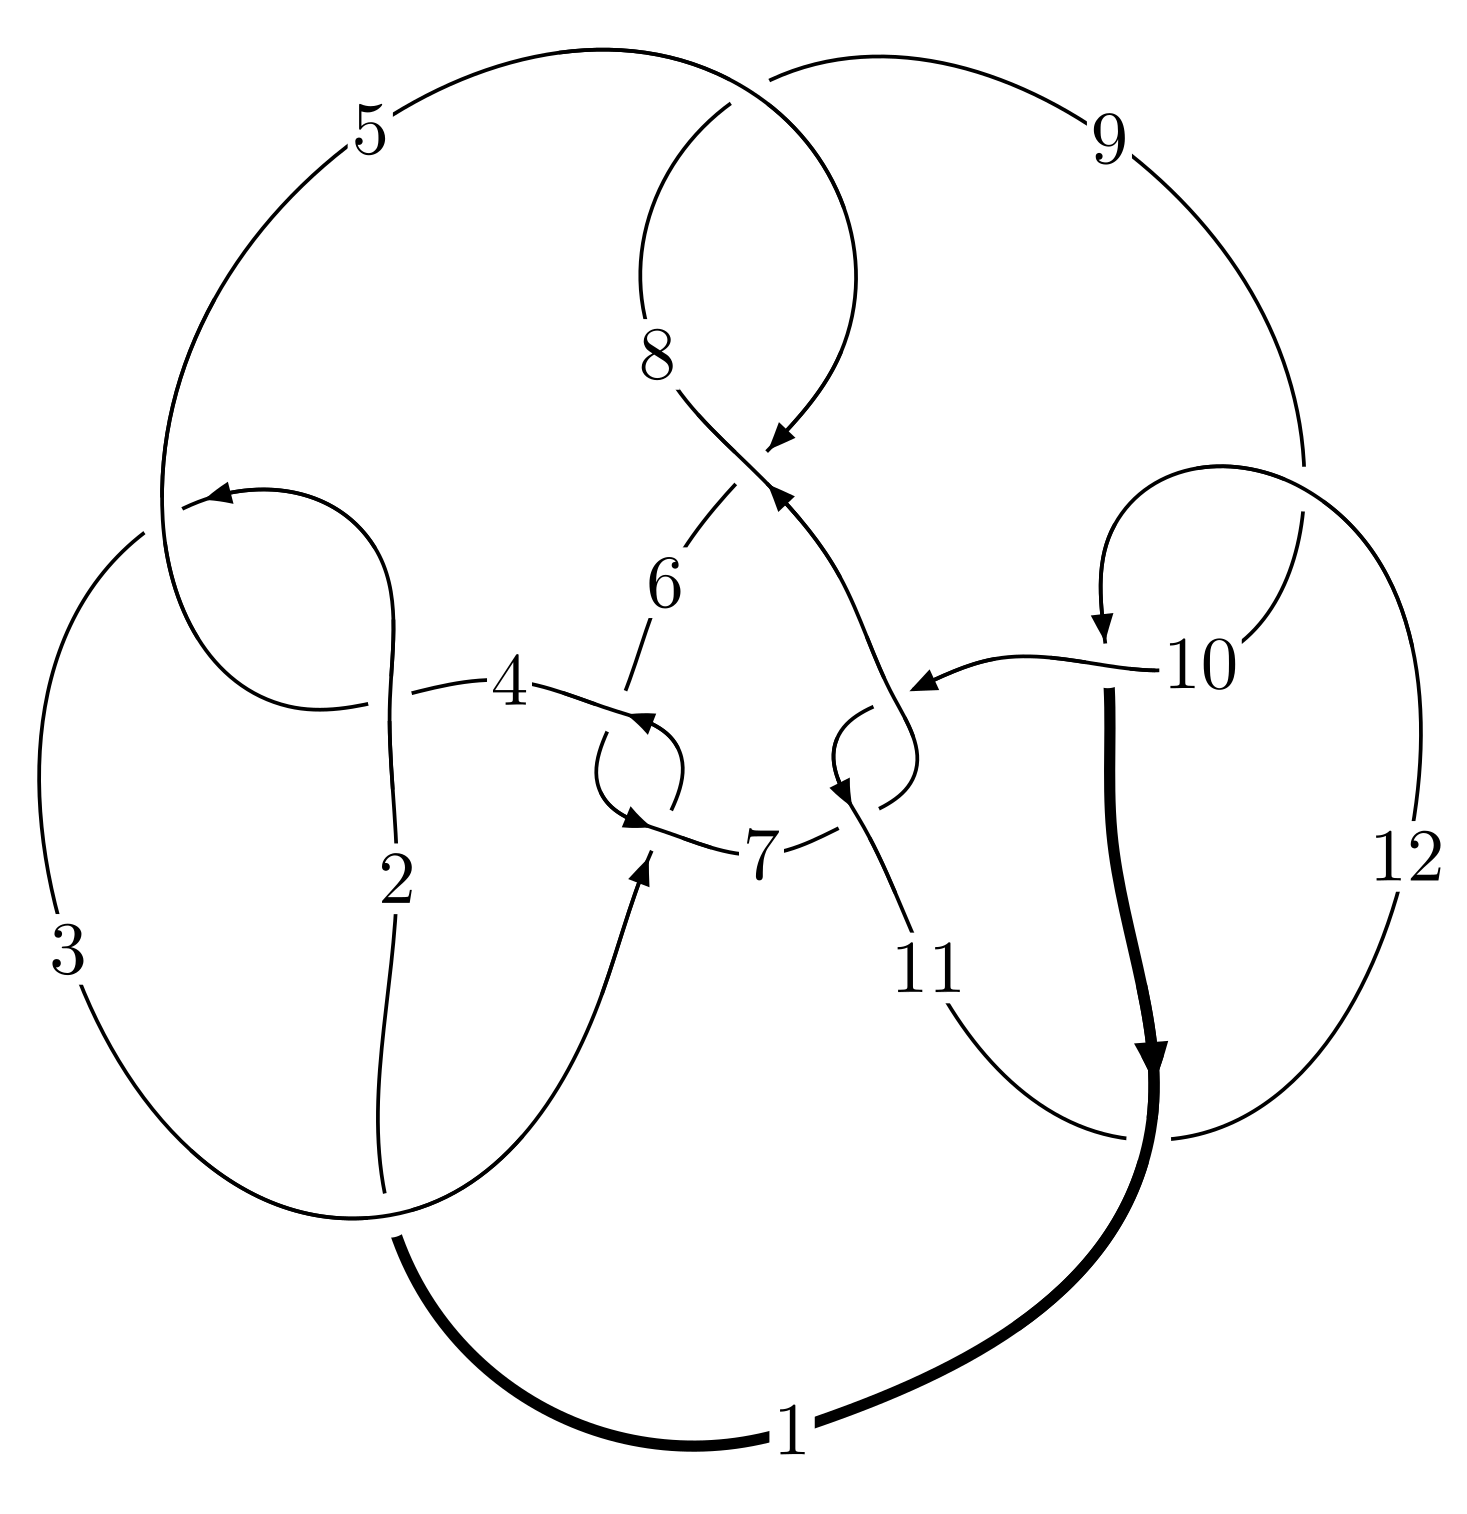
\includegraphics[width=112pt]{../../../GIT/diagram.site/Diagrams/png/2177_12n_0088.png}\\
\ \ \ A knot diagram\footnotemark}&
\allowdisplaybreaks
\textbf{Linearized knot diagam} \\
\cline{2-2}
 &
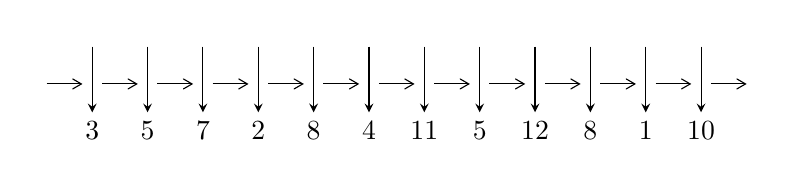
\begin{tikzpicture}[x=20pt, y=17pt]
	% nodes
	\node (C0) at (0, 0) {};
	\node (C1) at (1, 0) {};
	\node (C1U) at (1, +1) {};
	\node (C1D) at (1, -1) {3};

	\node (C2) at (2, 0) {};
	\node (C2U) at (2, +1) {};
	\node (C2D) at (2, -1) {5};

	\node (C3) at (3, 0) {};
	\node (C3U) at (3, +1) {};
	\node (C3D) at (3, -1) {7};

	\node (C4) at (4, 0) {};
	\node (C4U) at (4, +1) {};
	\node (C4D) at (4, -1) {2};

	\node (C5) at (5, 0) {};
	\node (C5U) at (5, +1) {};
	\node (C5D) at (5, -1) {8};

	\node (C6) at (6, 0) {};
	\node (C6U) at (6, +1) {};
	\node (C6D) at (6, -1) {4};

	\node (C7) at (7, 0) {};
	\node (C7U) at (7, +1) {};
	\node (C7D) at (7, -1) {11};

	\node (C8) at (8, 0) {};
	\node (C8U) at (8, +1) {};
	\node (C8D) at (8, -1) {5};

	\node (C9) at (9, 0) {};
	\node (C9U) at (9, +1) {};
	\node (C9D) at (9, -1) {12};

	\node (C10) at (10, 0) {};
	\node (C10U) at (10, +1) {};
	\node (C10D) at (10, -1) {8};

	\node (C11) at (11, 0) {};
	\node (C11U) at (11, +1) {};
	\node (C11D) at (11, -1) {1};

	\node (C12) at (12, 0) {};
	\node (C12U) at (12, +1) {};
	\node (C12D) at (12, -1) {10};
	\node (C13) at (13, 0) {};

	% arrows
	\draw[->,>={angle 60}]
	(C0) edge (C1) (C1) edge (C2) (C2) edge (C3) (C3) edge (C4) (C4) edge (C5) (C5) edge (C6) (C6) edge (C7) (C7) edge (C8) (C8) edge (C9) (C9) edge (C10) (C10) edge (C11) (C11) edge (C12) (C12) edge (C13) ;	\draw[->,>=stealth]
	(C1U) edge (C1D) (C2U) edge (C2D) (C3U) edge (C3D) (C4U) edge (C4D) (C5U) edge (C5D) (C6U) edge (C6D) (C7U) edge (C7D) (C8U) edge (C8D) (C9U) edge (C9D) (C10U) edge (C10D) (C11U) edge (C11D) (C12U) edge (C12D) ;
	\end{tikzpicture} \\
\hhline{~~} \\& 
\textbf{Solving Sequence} \\ \cline{2-2} 
 &
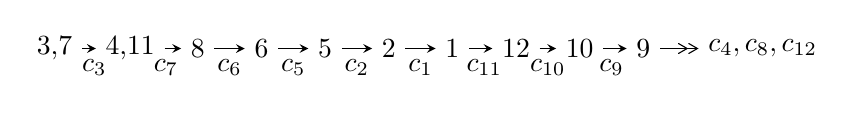
\begin{tikzpicture}[x=23pt, y=7pt]
	% node
	\node (A0) at (-1/8, 0) {3,7};
	\node (A1) at (17/16, 0) {4,11};
	\node (A2) at (17/8, 0) {8};
	\node (A3) at (25/8, 0) {6};
	\node (A4) at (33/8, 0) {5};
	\node (A5) at (41/8, 0) {2};
	\node (A6) at (49/8, 0) {1};
	\node (A7) at (57/8, 0) {12};
	\node (A8) at (65/8, 0) {10};
	\node (A9) at (73/8, 0) {9};
	\node (C1) at (1/2, -1) {$c_{3}$};
	\node (C2) at (13/8, -1) {$c_{7}$};
	\node (C3) at (21/8, -1) {$c_{6}$};
	\node (C4) at (29/8, -1) {$c_{5}$};
	\node (C5) at (37/8, -1) {$c_{2}$};
	\node (C6) at (45/8, -1) {$c_{1}$};
	\node (C7) at (53/8, -1) {$c_{11}$};
	\node (C8) at (61/8, -1) {$c_{10}$};
	\node (C9) at (69/8, -1) {$c_{9}$};
	\node (A10) at (11, 0) {$c_{4},c_{8},c_{12}$};

	% edge
	\draw[->,>=stealth]	
	(A0) edge (A1) (A1) edge (A2) (A2) edge (A3) (A3) edge (A4) (A4) edge (A5) (A5) edge (A6) (A6) edge (A7) (A7) edge (A8) (A8) edge (A9) ;
	\draw[->>,>={angle 60}]	
	(A9) edge (A10);
\end{tikzpicture} \\ 

\end{tabular} \\

\footnotetext{
The image of knot diagram is generated by the software ``\textbf{Draw programme}" developed by Andrew Bartholomew(\url{http://www.layer8.co.uk/maths/draw/index.htm\#Running-draw}), where we modified some parts for our purpose(\url{https://github.com/CATsTAILs/LinksPainter}).
}\phantom \\ \newline 
\centering \textbf{Ideals for irreducible components\footnotemark of $X_{\text{par}}$} 
 
\begin{align*}
I^u_{1}&=\langle 
1052 u^{13}+1602 u^{12}+\cdots+303 b+1332,\;a-1,\\
\phantom{I^u_{1}}&\phantom{= \langle  }u^{14}+u^{13}+2 u^{12}+u^{11}+6 u^{10}+4 u^9+4 u^8+u^7+6 u^6+4 u^5-2 u^3-4 u^2+4 u-1\rangle \\
I^u_{2}&=\langle 
-9.89889\times10^{121} u^{57}-3.65306\times10^{122} u^{56}+\cdots+1.87725\times10^{122} b+2.30550\times10^{123},\\
\phantom{I^u_{2}}&\phantom{= \langle  }-1.95314\times10^{123} u^{57}-7.22784\times10^{123} u^{56}+\cdots+3.00360\times10^{123} a+3.04298\times10^{124},\\
\phantom{I^u_{2}}&\phantom{= \langle  }u^{58}+4 u^{57}+\cdots-32 u-4\rangle \\
I^u_{3}&=\langle 
u^2+b+2,\;a+1,\;u^3- u^2+2 u-1\rangle \\
I^u_{4}&=\langle 
-2 a u+b+2 u-1,\;u^2 a+a^2- a u+3 u^2+a- u+5,\;u^3- u^2+2 u-1\rangle \\
I^u_{5}&=\langle 
b+2 u+3,\;a,\;u^2+u-1\rangle \\
\\
I^v_{1}&=\langle 
a,\;3 b+2 v+13,\;v^2+7 v+1\rangle \\
\end{align*}
\raggedright * 6 irreducible components of $\dim_{\mathbb{C}}=0$, with total 85 representations.\\
\footnotetext{All coefficients of polynomials are rational numbers. But the coefficients are sometimes approximated in decimal forms when there is not enough margin.}
\newpage
\renewcommand{\arraystretch}{1}
\centering \section*{I. $I^u_{1}= \langle 1052 u^{13}+1602 u^{12}+\cdots+303 b+1332,\;a-1,\;u^{14}+u^{13}+\cdots+4 u-1 \rangle$}
\flushleft \textbf{(i) Arc colorings}\\
\begin{tabular}{m{7pt} m{180pt} m{7pt} m{180pt} }
\flushright $a_{3}=$&$\begin{pmatrix}1\\0\end{pmatrix}$ \\
\flushright $a_{7}=$&$\begin{pmatrix}0\\u\end{pmatrix}$ \\
\flushright $a_{4}=$&$\begin{pmatrix}1\\u^2\end{pmatrix}$ \\
\flushright $a_{11}=$&$\begin{pmatrix}1\\-3.47195 u^{13}-5.28713 u^{12}+\cdots+16.2145 u-4.39604\end{pmatrix}$ \\
\flushright $a_{8}=$&$\begin{pmatrix}- u\\1.81518 u^{13}+2.61716 u^{12}+\cdots-8.49175 u+3.47195\end{pmatrix}$ \\
\flushright $a_{6}=$&$\begin{pmatrix}u\\u^3+u\end{pmatrix}$ \\
\flushright $a_{5}=$&$\begin{pmatrix}0.264026 u^{13}+0.356436 u^{12}+\cdots-0.392739 u+0.801980\\-0.276128 u^{13}-0.611661 u^{12}+\cdots+1.62046 u+0.179318\end{pmatrix}$ \\
\flushright $a_{2}=$&$\begin{pmatrix}0.264026 u^{13}+0.356436 u^{12}+\cdots-0.392739 u+0.801980\\0.375138 u^{13}+0.578658 u^{12}+\cdots-1.72607 u-0.0869087\end{pmatrix}$ \\
\flushright $a_{1}=$&$\begin{pmatrix}0.639164 u^{13}+0.935094 u^{12}+\cdots-2.11881 u+0.715072\\0.375138 u^{13}+0.578658 u^{12}+\cdots-1.72607 u-0.0869087\end{pmatrix}$ \\
\flushright $a_{12}=$&$\begin{pmatrix}0.106711 u^{13}+0.0385039 u^{12}+\cdots+0.567657 u+0.558856\\-3.35314 u^{13}-4.99340 u^{12}+\cdots+15.5545 u-4.81848\end{pmatrix}$ \\
\flushright $a_{10}=$&$\begin{pmatrix}u^2+1\\-4.27393 u^{13}-6.35314 u^{12}+\cdots+20.0033 u-6.21122\end{pmatrix}$ \\
\flushright $a_{9}=$&$\begin{pmatrix}0.573157 u^{13}+0.512651 u^{12}+\cdots-0.937294 u+1.09791\\-1.34103 u^{13}-2.07151 u^{12}+\cdots+6.66007 u-2.46645\end{pmatrix}$\\&\end{tabular}
\flushleft \textbf{(ii) Obstruction class $= -1$}\\~\\
\flushleft \textbf{(iii) Cusp Shapes $= \frac{1196}{303} u^{13}+\frac{1124}{101} u^{12}+\cdots-\frac{3188}{303} u-\frac{3026}{101}$}\\~\\
\newpage\renewcommand{\arraystretch}{1}
\flushleft \textbf{(iv) u-Polynomials at the component}\newline \\
\begin{tabular}{m{50pt}|m{274pt}}
Crossings & \hspace{64pt}u-Polynomials at each crossing \\
\hline $$\begin{aligned}c_{1},c_{11}\end{aligned}$$&$\begin{aligned}
&u^{14}+9 u^{13}+\cdots+16 u+1
\end{aligned}$\\
\hline $$\begin{aligned}c_{2},c_{4},c_{9}\\c_{12}\end{aligned}$$&$\begin{aligned}
&u^{14}-3 u^{13}+\cdots-2 u-1
\end{aligned}$\\
\hline $$\begin{aligned}c_{3},c_{6},c_{7}\\c_{10}\end{aligned}$$&$\begin{aligned}
&u^{14}- u^{13}+\cdots-4 u-1
\end{aligned}$\\
\hline $$\begin{aligned}c_{5},c_{8}\end{aligned}$$&$\begin{aligned}
&u^{14}-7 u^{13}+\cdots-24 u+8
\end{aligned}$\\
\hline
\end{tabular}\\~\\
\newpage\renewcommand{\arraystretch}{1}
\flushleft \textbf{(v) Riley Polynomials at the component}\newline \\
\begin{tabular}{m{50pt}|m{274pt}}
Crossings & \hspace{64pt}Riley Polynomials at each crossing \\
\hline $$\begin{aligned}c_{1},c_{11}\end{aligned}$$&$\begin{aligned}
&y^{14}-5 y^{13}+\cdots-208 y+1
\end{aligned}$\\
\hline $$\begin{aligned}c_{2},c_{4},c_{9}\\c_{12}\end{aligned}$$&$\begin{aligned}
&y^{14}-9 y^{13}+\cdots-16 y+1
\end{aligned}$\\
\hline $$\begin{aligned}c_{3},c_{6},c_{7}\\c_{10}\end{aligned}$$&$\begin{aligned}
&y^{14}+3 y^{13}+\cdots-8 y+1
\end{aligned}$\\
\hline $$\begin{aligned}c_{5},c_{8}\end{aligned}$$&$\begin{aligned}
&y^{14}-7 y^{13}+\cdots+384 y+64
\end{aligned}$\\
\hline
\end{tabular}\\~\\
\newpage\flushleft \textbf{(vi) Complex Volumes and Cusp Shapes}
$$\begin{array}{c|c|c}  
\text{Solutions to }I^u_{1}& \I (\text{vol} + \sqrt{-1}CS) & \text{Cusp shape}\\
 \hline 
\begin{aligned}
u &= -0.985278\phantom{ +0.000000I} \\
a &= \phantom{-}1.00000\phantom{ +0.000000I} \\
b &= \phantom{-}0.711293\phantom{ +0.000000I}\end{aligned}
 & -10.4546\phantom{ +0.000000I} & -24.6220\phantom{ +0.000000I} \\ \hline\begin{aligned}
u &= -0.336026 + 0.979953 I \\
a &= \phantom{-}1.00000\phantom{ +0.000000I} \\
b &= \phantom{-}0.255618 - 1.069010 I\end{aligned}
 & \phantom{-}3.75566 - 0.17244 I & -4.31674 + 1.33622 I \\ \hline\begin{aligned}
u &= -0.336026 - 0.979953 I \\
a &= \phantom{-}1.00000\phantom{ +0.000000I} \\
b &= \phantom{-}0.255618 + 1.069010 I\end{aligned}
 & \phantom{-}3.75566 + 0.17244 I & -4.31674 - 1.33622 I \\ \hline\begin{aligned}
u &= \phantom{-}0.811264 + 0.869909 I \\
a &= \phantom{-}1.00000\phantom{ +0.000000I} \\
b &= \phantom{-}0.73524 + 1.21182 I\end{aligned}
 & -1.53918 - 8.57795 I & -13.9694 + 8.6920 I \\ \hline\begin{aligned}
u &= \phantom{-}0.811264 - 0.869909 I \\
a &= \phantom{-}1.00000\phantom{ +0.000000I} \\
b &= \phantom{-}0.73524 - 1.21182 I\end{aligned}
 & -1.53918 + 8.57795 I & -13.9694 - 8.6920 I \\ \hline\begin{aligned}
u &= -0.920950 + 0.794472 I \\
a &= \phantom{-}1.00000\phantom{ +0.000000I} \\
b &= \phantom{-}2.22969 - 0.56400 I\end{aligned}
 & -7.24910 - 2.92807 I & -16.0849 + 1.6852 I \\ \hline\begin{aligned}
u &= -0.920950 - 0.794472 I \\
a &= \phantom{-}1.00000\phantom{ +0.000000I} \\
b &= \phantom{-}2.22969 + 0.56400 I\end{aligned}
 & -7.24910 + 2.92807 I & -16.0849 - 1.6852 I \\ \hline\begin{aligned}
u &= \phantom{-}0.685146 + 1.154840 I \\
a &= \phantom{-}1.00000\phantom{ +0.000000I} \\
b &= \phantom{-}1.095700 + 0.836675 I\end{aligned}
 & \phantom{-}1.33116 - 5.50874 I & -7.69545 + 3.70076 I \\ \hline\begin{aligned}
u &= \phantom{-}0.685146 - 1.154840 I \\
a &= \phantom{-}1.00000\phantom{ +0.000000I} \\
b &= \phantom{-}1.095700 - 0.836675 I\end{aligned}
 & \phantom{-}1.33116 + 5.50874 I & -7.69545 - 3.70076 I \\ \hline\begin{aligned}
u &= \phantom{-}0.495258\phantom{ +0.000000I} \\
a &= \phantom{-}1.00000\phantom{ +0.000000I} \\
b &= -0.192497\phantom{ +0.000000I}\end{aligned}
 & -0.942520\phantom{ +0.000000I} & -9.45120\phantom{ +0.000000I}\\
 \hline 
 \end{array}$$\newpage$$\begin{array}{c|c|c}  
\text{Solutions to }I^u_{1}& \I (\text{vol} + \sqrt{-1}CS) & \text{Cusp shape}\\
 \hline 
\begin{aligned}
u &= -0.90906 + 1.21001 I \\
a &= \phantom{-}1.00000\phantom{ +0.000000I} \\
b &= \phantom{-}1.54300 - 1.48268 I\end{aligned}
 & -4.9818 + 17.0516 I & -13.2441 - 9.4300 I \\ \hline\begin{aligned}
u &= -0.90906 - 1.21001 I \\
a &= \phantom{-}1.00000\phantom{ +0.000000I} \\
b &= \phantom{-}1.54300 + 1.48268 I\end{aligned}
 & -4.9818 - 17.0516 I & -13.2441 + 9.4300 I \\ \hline\begin{aligned}
u &= \phantom{-}0.414634 + 0.221302 I \\
a &= \phantom{-}1.00000\phantom{ +0.000000I} \\
b &= \phantom{-}3.88135 + 1.29131 I\end{aligned}
 & -2.88995 + 0.46660 I & -33.6526 + 15.6404 I \\ \hline\begin{aligned}
u &= \phantom{-}0.414634 - 0.221302 I \\
a &= \phantom{-}1.00000\phantom{ +0.000000I} \\
b &= \phantom{-}3.88135 - 1.29131 I\end{aligned}
 & -2.88995 - 0.46660 I & -33.6526 - 15.6404 I\\
 \hline 
 \end{array}$$\newpage\newpage\renewcommand{\arraystretch}{1}
\centering \section*{II. $I^u_{2}= \langle -9.90\times10^{121} u^{57}-3.65\times10^{122} u^{56}+\cdots+1.88\times10^{122} b+2.31\times10^{123},\;-1.95\times10^{123} u^{57}-7.23\times10^{123} u^{56}+\cdots+3.00\times10^{123} a+3.04\times10^{124},\;u^{58}+4 u^{57}+\cdots-32 u-4 \rangle$}
\flushleft \textbf{(i) Arc colorings}\\
\begin{tabular}{m{7pt} m{180pt} m{7pt} m{180pt} }
\flushright $a_{3}=$&$\begin{pmatrix}1\\0\end{pmatrix}$ \\
\flushright $a_{7}=$&$\begin{pmatrix}0\\u\end{pmatrix}$ \\
\flushright $a_{4}=$&$\begin{pmatrix}1\\u^2\end{pmatrix}$ \\
\flushright $a_{11}=$&$\begin{pmatrix}0.650266 u^{57}+2.40639 u^{56}+\cdots-29.2651 u-10.1311\\0.527307 u^{57}+1.94596 u^{56}+\cdots-22.7262 u-12.2812\end{pmatrix}$ \\
\flushright $a_{8}=$&$\begin{pmatrix}0.436407 u^{57}+1.53830 u^{56}+\cdots-28.9670 u-2.62090\\-0.0748277 u^{57}-0.332438 u^{56}+\cdots-0.473003 u+4.86221\end{pmatrix}$ \\
\flushright $a_{6}=$&$\begin{pmatrix}u\\u^3+u\end{pmatrix}$ \\
\flushright $a_{5}=$&$\begin{pmatrix}-1.28188 u^{57}-4.65236 u^{56}+\cdots+75.0228 u+14.7864\\-0.168206 u^{57}-0.619830 u^{56}+\cdots+8.16456 u+2.60510\end{pmatrix}$ \\
\flushright $a_{2}=$&$\begin{pmatrix}-1.28188 u^{57}-4.65236 u^{56}+\cdots+75.0228 u+14.7864\\-0.0117219 u^{57}-0.0393795 u^{56}+\cdots+1.91334 u-0.704417\end{pmatrix}$ \\
\flushright $a_{1}=$&$\begin{pmatrix}-1.29360 u^{57}-4.69174 u^{56}+\cdots+76.9361 u+14.0819\\-0.0117219 u^{57}-0.0393795 u^{56}+\cdots+1.91334 u-0.704417\end{pmatrix}$ \\
\flushright $a_{12}=$&$\begin{pmatrix}-2.62838 u^{57}-9.50925 u^{56}+\cdots+161.265 u+25.9962\\0.376226 u^{57}+1.39349 u^{56}+\cdots-13.2103 u-10.9310\end{pmatrix}$ \\
\flushright $a_{10}=$&$\begin{pmatrix}1.25102 u^{57}+4.66027 u^{56}+\cdots-63.7398 u-18.6633\\0.372290 u^{57}+1.46092 u^{56}+\cdots-14.4154 u-13.9819\end{pmatrix}$ \\
\flushright $a_{9}=$&$\begin{pmatrix}-3.61469 u^{57}-13.0974 u^{56}+\cdots+213.519 u+37.6085\\-0.129312 u^{57}-0.407792 u^{56}+\cdots+12.1768 u-2.92917\end{pmatrix}$\\&\end{tabular}
\flushleft \textbf{(ii) Obstruction class $= -1$}\\~\\
\flushleft \textbf{(iii) Cusp Shapes $= 8.07218 u^{57}+30.8062 u^{56}+\cdots-296.329 u-286.736$}\\~\\
\newpage\renewcommand{\arraystretch}{1}
\flushleft \textbf{(iv) u-Polynomials at the component}\newline \\
\begin{tabular}{m{50pt}|m{274pt}}
Crossings & \hspace{64pt}u-Polynomials at each crossing \\
\hline $$\begin{aligned}c_{1},c_{11}\end{aligned}$$&$\begin{aligned}
&u^{58}+32 u^{57}+\cdots+25 u+1
\end{aligned}$\\
\hline $$\begin{aligned}c_{2},c_{4},c_{9}\\c_{12}\end{aligned}$$&$\begin{aligned}
&u^{58}-4 u^{57}+\cdots+5 u+1
\end{aligned}$\\
\hline $$\begin{aligned}c_{3},c_{6},c_{7}\\c_{10}\end{aligned}$$&$\begin{aligned}
&u^{58}-4 u^{57}+\cdots+32 u-4
\end{aligned}$\\
\hline $$\begin{aligned}c_{5},c_{8}\end{aligned}$$&$\begin{aligned}
&(u^{29}+2 u^{28}+\cdots-28 u-8)^{2}
\end{aligned}$\\
\hline
\end{tabular}\\~\\
\newpage\renewcommand{\arraystretch}{1}
\flushleft \textbf{(v) Riley Polynomials at the component}\newline \\
\begin{tabular}{m{50pt}|m{274pt}}
Crossings & \hspace{64pt}Riley Polynomials at each crossing \\
\hline $$\begin{aligned}c_{1},c_{11}\end{aligned}$$&$\begin{aligned}
&y^{58}-8 y^{57}+\cdots+195 y+1
\end{aligned}$\\
\hline $$\begin{aligned}c_{2},c_{4},c_{9}\\c_{12}\end{aligned}$$&$\begin{aligned}
&y^{58}-32 y^{57}+\cdots-25 y+1
\end{aligned}$\\
\hline $$\begin{aligned}c_{3},c_{6},c_{7}\\c_{10}\end{aligned}$$&$\begin{aligned}
&y^{58}+18 y^{57}+\cdots-984 y+16
\end{aligned}$\\
\hline $$\begin{aligned}c_{5},c_{8}\end{aligned}$$&$\begin{aligned}
&(y^{29}-28 y^{28}+\cdots+2896 y-64)^{2}
\end{aligned}$\\
\hline
\end{tabular}\\~\\
\newpage\flushleft \textbf{(vi) Complex Volumes and Cusp Shapes}
$$\begin{array}{c|c|c}  
\text{Solutions to }I^u_{2}& \I (\text{vol} + \sqrt{-1}CS) & \text{Cusp shape}\\
 \hline 
\begin{aligned}
u &= -0.721948 + 0.675707 I \\
a &= -1.050020 + 0.447654 I \\
b &= -0.511195 + 1.317100 I\end{aligned}
 & \phantom{-}2.03816 + 4.43643 I & -7.12586 - 5.70665 I \\ \hline\begin{aligned}
u &= -0.721948 - 0.675707 I \\
a &= -1.050020 - 0.447654 I \\
b &= -0.511195 - 1.317100 I\end{aligned}
 & \phantom{-}2.03816 - 4.43643 I & -7.12586 + 5.70665 I \\ \hline\begin{aligned}
u &= -0.244212 + 0.907147 I \\
a &= -1.73124 + 0.12831 I \\
b &= -0.254583 + 0.569117 I\end{aligned}
 & \phantom{-}4.34822 + 5.30129 I & -10.14110 - 5.91971 I \\ \hline\begin{aligned}
u &= -0.244212 - 0.907147 I \\
a &= -1.73124 - 0.12831 I \\
b &= -0.254583 - 0.569117 I\end{aligned}
 & \phantom{-}4.34822 - 5.30129 I & -10.14110 + 5.91971 I \\ \hline\begin{aligned}
u &= \phantom{-}0.578373 + 0.893018 I \\
a &= -0.516169 - 0.639005 I \\
b &= \phantom{-}0.175167 - 1.077130 I\end{aligned}
 & -1.15248 + 2.97907 I & -12.00000 + 0. I\phantom{ +0.000000I} \\ \hline\begin{aligned}
u &= \phantom{-}0.578373 - 0.893018 I \\
a &= -0.516169 + 0.639005 I \\
b &= \phantom{-}0.175167 + 1.077130 I\end{aligned}
 & -1.15248 - 2.97907 I & -12.00000 + 0. I\phantom{ +0.000000I} \\ \hline\begin{aligned}
u &= -0.676773 + 0.824397 I \\
a &= -0.377087 - 1.293150 I \\
b &= -0.982001 + 0.458444 I\end{aligned}
 & -4.05295 + 3.42058 I & -12.00000 + 0. I\phantom{ +0.000000I} \\ \hline\begin{aligned}
u &= -0.676773 - 0.824397 I \\
a &= -0.377087 + 1.293150 I \\
b &= -0.982001 - 0.458444 I\end{aligned}
 & -4.05295 - 3.42058 I & -12.00000 + 0. I\phantom{ +0.000000I} \\ \hline\begin{aligned}
u &= \phantom{-}0.978563 + 0.440662 I \\
a &= \phantom{-}0.331345 + 0.627843 I \\
b &= -0.228672 + 1.138160 I\end{aligned}
 & -0.488787 - 0.370462 I & -12.00000 + 0. I\phantom{ +0.000000I} \\ \hline\begin{aligned}
u &= \phantom{-}0.978563 - 0.440662 I \\
a &= \phantom{-}0.331345 - 0.627843 I \\
b &= -0.228672 - 1.138160 I\end{aligned}
 & -0.488787 + 0.370462 I & -12.00000 + 0. I\phantom{ +0.000000I}\\
 \hline 
 \end{array}$$\newpage$$\begin{array}{c|c|c}  
\text{Solutions to }I^u_{2}& \I (\text{vol} + \sqrt{-1}CS) & \text{Cusp shape}\\
 \hline 
\begin{aligned}
u &= -0.012023 + 0.920805 I \\
a &= \phantom{-}1.65342 - 0.02280 I \\
b &= \phantom{-}0.209786 - 0.307915 I\end{aligned}
 & \phantom{-}4.90257 - 1.34329 I & -7.80264 + 1.36225 I \\ \hline\begin{aligned}
u &= -0.012023 - 0.920805 I \\
a &= \phantom{-}1.65342 + 0.02280 I \\
b &= \phantom{-}0.209786 + 0.307915 I\end{aligned}
 & \phantom{-}4.90257 + 1.34329 I & -7.80264 - 1.36225 I \\ \hline\begin{aligned}
u &= -0.580576 + 0.921658 I \\
a &= -1.003690 - 0.228249 I \\
b &= -1.66287 + 0.18113 I\end{aligned}
 & -3.74876 + 1.54341 I & \phantom{-0.000000 } 0 \\ \hline\begin{aligned}
u &= -0.580576 - 0.921658 I \\
a &= -1.003690 + 0.228249 I \\
b &= -1.66287 - 0.18113 I\end{aligned}
 & -3.74876 - 1.54341 I & \phantom{-0.000000 } 0 \\ \hline\begin{aligned}
u &= \phantom{-}0.793089 + 0.792547 I \\
a &= -0.947329 - 0.215431 I \\
b &= -1.66287 - 0.18113 I\end{aligned}
 & -3.74876 - 1.54341 I & \phantom{-0.000000 } 0 \\ \hline\begin{aligned}
u &= \phantom{-}0.793089 - 0.792547 I \\
a &= -0.947329 + 0.215431 I \\
b &= -1.66287 + 0.18113 I\end{aligned}
 & -3.74876 + 1.54341 I & \phantom{-0.000000 } 0 \\ \hline\begin{aligned}
u &= \phantom{-}0.272105 + 0.830532 I \\
a &= -0.764969 - 0.947014 I \\
b &= \phantom{-}0.175167 + 1.077130 I\end{aligned}
 & -1.15248 - 2.97907 I & -9.53425 + 4.84429 I \\ \hline\begin{aligned}
u &= \phantom{-}0.272105 - 0.830532 I \\
a &= -0.764969 + 0.947014 I \\
b &= \phantom{-}0.175167 - 1.077130 I\end{aligned}
 & -1.15248 + 2.97907 I & -9.53425 - 4.84429 I \\ \hline\begin{aligned}
u &= \phantom{-}0.455577 + 1.032690 I \\
a &= -0.805887 + 0.343573 I \\
b &= -0.511195 - 1.317100 I\end{aligned}
 & \phantom{-}2.03816 - 4.43643 I & \phantom{-0.000000 } 0 \\ \hline\begin{aligned}
u &= \phantom{-}0.455577 - 1.032690 I \\
a &= -0.805887 - 0.343573 I \\
b &= -0.511195 + 1.317100 I\end{aligned}
 & \phantom{-}2.03816 + 4.43643 I & \phantom{-0.000000 } 0\\
 \hline 
 \end{array}$$\newpage$$\begin{array}{c|c|c}  
\text{Solutions to }I^u_{2}& \I (\text{vol} + \sqrt{-1}CS) & \text{Cusp shape}\\
 \hline 
\begin{aligned}
u &= -0.802696 + 0.874767 I \\
a &= -0.085771 + 0.996315 I \\
b &= \phantom{-}0.307471\phantom{ +0.000000I}\end{aligned}
 & -7.39364\phantom{ +0.000000I} & \phantom{-0.000000 } 0 \\ \hline\begin{aligned}
u &= -0.802696 - 0.874767 I \\
a &= -0.085771 - 0.996315 I \\
b &= \phantom{-}0.307471\phantom{ +0.000000I}\end{aligned}
 & -7.39364\phantom{ +0.000000I} & \phantom{-0.000000 } 0 \\ \hline\begin{aligned}
u &= -1.031050 + 0.638573 I \\
a &= -0.116942 - 1.016090 I \\
b &= -0.777038 - 0.585721 I\end{aligned}
 & -3.19564 - 4.35308 I & \phantom{-0.000000 } 0 \\ \hline\begin{aligned}
u &= -1.031050 - 0.638573 I \\
a &= -0.116942 + 1.016090 I \\
b &= -0.777038 + 0.585721 I\end{aligned}
 & -3.19564 + 4.35308 I & \phantom{-0.000000 } 0 \\ \hline\begin{aligned}
u &= -0.797235 + 0.914221 I \\
a &= \phantom{-}1.140830 - 0.268629 I \\
b &= \phantom{-}1.25483 - 0.74117 I\end{aligned}
 & -7.27243 + 6.00653 I & \phantom{-0.000000 } 0 \\ \hline\begin{aligned}
u &= -0.797235 - 0.914221 I \\
a &= \phantom{-}1.140830 + 0.268629 I \\
b &= \phantom{-}1.25483 + 0.74117 I\end{aligned}
 & -7.27243 - 6.00653 I & \phantom{-0.000000 } 0 \\ \hline\begin{aligned}
u &= \phantom{-}0.047575 + 0.760395 I \\
a &= \phantom{-}0.657460 - 1.245780 I \\
b &= -0.228672 + 1.138160 I\end{aligned}
 & -0.488787 - 0.370462 I & -8.36692 + 2.50640 I \\ \hline\begin{aligned}
u &= \phantom{-}0.047575 - 0.760395 I \\
a &= \phantom{-}0.657460 + 1.245780 I \\
b &= -0.228672 - 1.138160 I\end{aligned}
 & -0.488787 + 0.370462 I & -8.36692 - 2.50640 I \\ \hline\begin{aligned}
u &= \phantom{-}0.769423 + 0.972965 I \\
a &= -0.111786 + 0.971295 I \\
b &= -0.777038 - 0.585721 I\end{aligned}
 & -3.19564 - 4.35308 I & \phantom{-0.000000 } 0 \\ \hline\begin{aligned}
u &= \phantom{-}0.769423 - 0.972965 I \\
a &= -0.111786 - 0.971295 I \\
b &= -0.777038 + 0.585721 I\end{aligned}
 & -3.19564 + 4.35308 I & \phantom{-0.000000 } 0\\
 \hline 
 \end{array}$$\newpage$$\begin{array}{c|c|c}  
\text{Solutions to }I^u_{2}& \I (\text{vol} + \sqrt{-1}CS) & \text{Cusp shape}\\
 \hline 
\begin{aligned}
u &= -0.824653 + 1.012890 I \\
a &= \phantom{-}0.164016 + 1.106820 I \\
b &= \phantom{-}1.240200 - 0.434590 I\end{aligned}
 & -6.56035 + 9.36152 I & \phantom{-0.000000 } 0 \\ \hline\begin{aligned}
u &= -0.824653 - 1.012890 I \\
a &= \phantom{-}0.164016 - 1.106820 I \\
b &= \phantom{-}1.240200 + 0.434590 I\end{aligned}
 & -6.56035 - 9.36152 I & \phantom{-0.000000 } 0 \\ \hline\begin{aligned}
u &= \phantom{-}0.202324 + 1.331240 I \\
a &= -0.027585 + 0.375583 I \\
b &= -0.20707 - 3.33341 I\end{aligned}
 & \phantom{-}1.81502 - 2.87998 I & \phantom{-0.000000 } 0 \\ \hline\begin{aligned}
u &= \phantom{-}0.202324 - 1.331240 I \\
a &= -0.027585 - 0.375583 I \\
b &= -0.20707 + 3.33341 I\end{aligned}
 & \phantom{-}1.81502 + 2.87998 I & \phantom{-0.000000 } 0 \\ \hline\begin{aligned}
u &= -0.803948 + 1.131230 I \\
a &= -1.108550 + 0.044327 I \\
b &= -1.28128 + 1.27353 I\end{aligned}
 & -1.66044 + 11.01250 I & \phantom{-0.000000 } 0 \\ \hline\begin{aligned}
u &= -0.803948 - 1.131230 I \\
a &= -1.108550 - 0.044327 I \\
b &= -1.28128 - 1.27353 I\end{aligned}
 & -1.66044 - 11.01250 I & \phantom{-0.000000 } 0 \\ \hline\begin{aligned}
u &= \phantom{-}0.601388\phantom{ +0.000000I} \\
a &= -0.244736\phantom{ +0.000000I} \\
b &= -7.40752\phantom{ +0.000000I}\end{aligned}
 & -2.67255\phantom{ +0.000000I} & -211.680\phantom{ +0.000000I} \\ \hline\begin{aligned}
u &= \phantom{-}0.557093 + 0.195871 I \\
a &= \phantom{-}0.779962 - 0.625827 I \\
b &= -0.0910519\phantom{ +0.000000I}\end{aligned}
 & -0.942618\phantom{ +0.000000I} & -9.31087 + 0. I\phantom{ +0.000000I} \\ \hline\begin{aligned}
u &= \phantom{-}0.557093 - 0.195871 I \\
a &= \phantom{-}0.779962 + 0.625827 I \\
b &= -0.0910519\phantom{ +0.000000I}\end{aligned}
 & -0.942618\phantom{ +0.000000I} & -9.31087 + 0. I\phantom{ +0.000000I} \\ \hline\begin{aligned}
u &= -0.66392 + 1.25713 I \\
a &= \phantom{-}0.830507 + 0.195558 I \\
b &= \phantom{-}1.25483 - 0.74117 I\end{aligned}
 & -7.27243 + 6.00653 I & \phantom{-0.000000 } 0\\
 \hline 
 \end{array}$$\newpage$$\begin{array}{c|c|c}  
\text{Solutions to }I^u_{2}& \I (\text{vol} + \sqrt{-1}CS) & \text{Cusp shape}\\
 \hline 
\begin{aligned}
u &= -0.66392 - 1.25713 I \\
a &= \phantom{-}0.830507 - 0.195558 I \\
b &= \phantom{-}1.25483 + 0.74117 I\end{aligned}
 & -7.27243 - 6.00653 I & \phantom{-0.000000 } 0 \\ \hline\begin{aligned}
u &= \phantom{-}1.32127 + 0.56430 I \\
a &= -0.207826 + 0.712702 I \\
b &= -0.982001 + 0.458444 I\end{aligned}
 & -4.05295 + 3.42058 I & \phantom{-0.000000 } 0 \\ \hline\begin{aligned}
u &= \phantom{-}1.32127 - 0.56430 I \\
a &= -0.207826 - 0.712702 I \\
b &= -0.982001 - 0.458444 I\end{aligned}
 & -4.05295 - 3.42058 I & \phantom{-0.000000 } 0 \\ \hline\begin{aligned}
u &= -1.25634 + 0.74661 I \\
a &= \phantom{-}0.131009 + 0.884078 I \\
b &= \phantom{-}1.240200 + 0.434590 I\end{aligned}
 & -6.56035 - 9.36152 I & \phantom{-0.000000 } 0 \\ \hline\begin{aligned}
u &= -1.25634 - 0.74661 I \\
a &= \phantom{-}0.131009 - 0.884078 I \\
b &= \phantom{-}1.240200 - 0.434590 I\end{aligned}
 & -6.56035 + 9.36152 I & \phantom{-0.000000 } 0 \\ \hline\begin{aligned}
u &= \phantom{-}0.513312 + 0.101132 I \\
a &= \phantom{-}0.925268 - 0.379313 I \\
b &= -0.165385\phantom{ +0.000000I}\end{aligned}
 & -0.942376\phantom{ +0.000000I} & -9.38299 + 0. I\phantom{ +0.000000I} \\ \hline\begin{aligned}
u &= \phantom{-}0.513312 - 0.101132 I \\
a &= \phantom{-}0.925268 + 0.379313 I \\
b &= -0.165385\phantom{ +0.000000I}\end{aligned}
 & -0.942376\phantom{ +0.000000I} & -9.38299 + 0. I\phantom{ +0.000000I} \\ \hline\begin{aligned}
u &= -0.505572 + 0.039267 I \\
a &= -0.19450 - 2.64824 I \\
b &= -0.20707 - 3.33341 I\end{aligned}
 & \phantom{-}1.81502 - 2.87998 I & -58.6220 + 17.5185 I \\ \hline\begin{aligned}
u &= -0.505572 - 0.039267 I \\
a &= -0.19450 + 2.64824 I \\
b &= -0.20707 + 3.33341 I\end{aligned}
 & \phantom{-}1.81502 + 2.87998 I & -58.6220 - 17.5185 I \\ \hline\begin{aligned}
u &= \phantom{-}0.00112 + 1.52275 I \\
a &= \phantom{-}0.604691 + 0.008340 I \\
b &= \phantom{-}0.209786 - 0.307915 I\end{aligned}
 & \phantom{-}4.90257 - 1.34329 I & \phantom{-0.000000 } 0\\
 \hline 
 \end{array}$$\newpage$$\begin{array}{c|c|c}  
\text{Solutions to }I^u_{2}& \I (\text{vol} + \sqrt{-1}CS) & \text{Cusp shape}\\
 \hline 
\begin{aligned}
u &= \phantom{-}0.00112 - 1.52275 I \\
a &= \phantom{-}0.604691 - 0.008340 I \\
b &= \phantom{-}0.209786 + 0.307915 I\end{aligned}
 & \phantom{-}4.90257 + 1.34329 I & \phantom{-0.000000 } 0 \\ \hline\begin{aligned}
u &= -1.52437\phantom{ +0.000000I} \\
a &= \phantom{-}0.237820\phantom{ +0.000000I} \\
b &= \phantom{-}0.405949\phantom{ +0.000000I}\end{aligned}
 & -10.6310\phantom{ +0.000000I} & \phantom{-0.000000 } 0 \\ \hline\begin{aligned}
u &= \phantom{-}0.84107 + 1.28967 I \\
a &= -0.900638 + 0.036014 I \\
b &= -1.28128 - 1.27353 I\end{aligned}
 & -1.66044 - 11.01250 I & \phantom{-0.000000 } 0 \\ \hline\begin{aligned}
u &= \phantom{-}0.84107 - 1.28967 I \\
a &= -0.900638 - 0.036014 I \\
b &= -1.28128 + 1.27353 I\end{aligned}
 & -1.66044 + 11.01250 I & \phantom{-0.000000 } 0 \\ \hline\begin{aligned}
u &= \phantom{-}0.30639 + 1.60183 I \\
a &= -0.574465 + 0.042578 I \\
b &= -0.254583 - 0.569117 I\end{aligned}
 & \phantom{-}4.34822 - 5.30129 I & \phantom{-0.000000 } 0 \\ \hline\begin{aligned}
u &= \phantom{-}0.30639 - 1.60183 I \\
a &= -0.574465 - 0.042578 I \\
b &= -0.254583 + 0.569117 I\end{aligned}
 & \phantom{-}4.34822 + 5.30129 I & \phantom{-0.000000 } 0 \\ \hline\begin{aligned}
u &= -0.362526\phantom{ +0.000000I} \\
a &= \phantom{-}4.20485\phantom{ +0.000000I} \\
b &= \phantom{-}0.405949\phantom{ +0.000000I}\end{aligned}
 & -10.6310\phantom{ +0.000000I} & -48.5360\phantom{ +0.000000I} \\ \hline\begin{aligned}
u &= -0.147181\phantom{ +0.000000I} \\
a &= -4.08603\phantom{ +0.000000I} \\
b &= -7.40752\phantom{ +0.000000I}\end{aligned}
 & -2.67255\phantom{ +0.000000I} & -211.680\phantom{ +0.000000I}\\
 \hline 
 \end{array}$$\newpage\newpage\renewcommand{\arraystretch}{1}
\centering \section*{III. $I^u_{3}= \langle u^2+b+2,\;a+1,\;u^3- u^2+2 u-1 \rangle$}
\flushleft \textbf{(i) Arc colorings}\\
\begin{tabular}{m{7pt} m{180pt} m{7pt} m{180pt} }
\flushright $a_{3}=$&$\begin{pmatrix}1\\0\end{pmatrix}$ \\
\flushright $a_{7}=$&$\begin{pmatrix}0\\u\end{pmatrix}$ \\
\flushright $a_{4}=$&$\begin{pmatrix}1\\u^2\end{pmatrix}$ \\
\flushright $a_{11}=$&$\begin{pmatrix}-1\\- u^2-2\end{pmatrix}$ \\
\flushright $a_{8}=$&$\begin{pmatrix}- u\\- u^2+u-1\end{pmatrix}$ \\
\flushright $a_{6}=$&$\begin{pmatrix}u\\u^2- u+1\end{pmatrix}$ \\
\flushright $a_{5}=$&$\begin{pmatrix}u\\u^2- u+1\end{pmatrix}$ \\
\flushright $a_{2}=$&$\begin{pmatrix}u\\- u\end{pmatrix}$ \\
\flushright $a_{1}=$&$\begin{pmatrix}0\\- u\end{pmatrix}$ \\
\flushright $a_{12}=$&$\begin{pmatrix}-1\\-2 u^2-2\end{pmatrix}$ \\
\flushright $a_{10}=$&$\begin{pmatrix}- u^2-1\\- u^2+u-3\end{pmatrix}$ \\
\flushright $a_{9}=$&$\begin{pmatrix}- u\\- u^2+u-1\end{pmatrix}$\\&\end{tabular}
\flushleft \textbf{(ii) Obstruction class $= 1$}\\~\\
\flushleft \textbf{(iii) Cusp Shapes $= -8 u^2+8 u-20$}\\~\\
\newpage\renewcommand{\arraystretch}{1}
\flushleft \textbf{(iv) u-Polynomials at the component}\newline \\
\begin{tabular}{m{50pt}|m{274pt}}
Crossings & \hspace{64pt}u-Polynomials at each crossing \\
\hline $$\begin{aligned}c_{1},c_{3},c_{7}\\c_{11}\end{aligned}$$&$\begin{aligned}
&u^3- u^2+2 u-1
\end{aligned}$\\
\hline $$\begin{aligned}c_{2},c_{9}\end{aligned}$$&$\begin{aligned}
&u^3+u^2-1
\end{aligned}$\\
\hline $$\begin{aligned}c_{4},c_{12}\end{aligned}$$&$\begin{aligned}
&u^3- u^2+1
\end{aligned}$\\
\hline $$\begin{aligned}c_{5},c_{8}\end{aligned}$$&$\begin{aligned}
&u^3
\end{aligned}$\\
\hline $$\begin{aligned}c_{6},c_{10}\end{aligned}$$&$\begin{aligned}
&u^3+u^2+2 u+1
\end{aligned}$\\
\hline
\end{tabular}\\~\\
\newpage\renewcommand{\arraystretch}{1}
\flushleft \textbf{(v) Riley Polynomials at the component}\newline \\
\begin{tabular}{m{50pt}|m{274pt}}
Crossings & \hspace{64pt}Riley Polynomials at each crossing \\
\hline $$\begin{aligned}c_{1},c_{3},c_{6}\\c_{7},c_{10},c_{11}\end{aligned}$$&$\begin{aligned}
&y^3+3 y^2+2 y-1
\end{aligned}$\\
\hline $$\begin{aligned}c_{2},c_{4},c_{9}\\c_{12}\end{aligned}$$&$\begin{aligned}
&y^3- y^2+2 y-1
\end{aligned}$\\
\hline $$\begin{aligned}c_{5},c_{8}\end{aligned}$$&$\begin{aligned}
&y^3
\end{aligned}$\\
\hline
\end{tabular}\\~\\
\newpage\flushleft \textbf{(vi) Complex Volumes and Cusp Shapes}
$$\begin{array}{c|c|c}  
\text{Solutions to }I^u_{3}& \I (\text{vol} + \sqrt{-1}CS) & \text{Cusp shape}\\
 \hline 
\begin{aligned}
u &= \phantom{-}0.215080 + 1.307140 I \\
a &= -1.00000\phantom{ +0.000000I} \\
b &= -0.337641 - 0.562280 I\end{aligned}
 & \phantom{-}6.04826 - 5.65624 I & -4.98049 + 5.95889 I \\ \hline\begin{aligned}
u &= \phantom{-}0.215080 - 1.307140 I \\
a &= -1.00000\phantom{ +0.000000I} \\
b &= -0.337641 + 0.562280 I\end{aligned}
 & \phantom{-}6.04826 + 5.65624 I & -4.98049 - 5.95889 I \\ \hline\begin{aligned}
u &= \phantom{-}0.569840\phantom{ +0.000000I} \\
a &= -1.00000\phantom{ +0.000000I} \\
b &= -2.32472\phantom{ +0.000000I}\end{aligned}
 & -2.22691\phantom{ +0.000000I} & -18.0390\phantom{ +0.000000I}\\
 \hline 
 \end{array}$$\newpage\newpage\renewcommand{\arraystretch}{1}
\centering \section*{IV. $I^u_{4}= \langle -2 a u+b+2 u-1,\;u^2 a+a^2- a u+3 u^2+a- u+5,\;u^3- u^2+2 u-1 \rangle$}
\flushleft \textbf{(i) Arc colorings}\\
\begin{tabular}{m{7pt} m{180pt} m{7pt} m{180pt} }
\flushright $a_{3}=$&$\begin{pmatrix}1\\0\end{pmatrix}$ \\
\flushright $a_{7}=$&$\begin{pmatrix}0\\u\end{pmatrix}$ \\
\flushright $a_{4}=$&$\begin{pmatrix}1\\u^2\end{pmatrix}$ \\
\flushright $a_{11}=$&$\begin{pmatrix}a\\2 a u-2 u+1\end{pmatrix}$ \\
\flushright $a_{8}=$&$\begin{pmatrix}- a u+2 u^2+a- u+3\\a u+2 u^2- u+4\end{pmatrix}$ \\
\flushright $a_{6}=$&$\begin{pmatrix}u\\u^2- u+1\end{pmatrix}$ \\
\flushright $a_{5}=$&$\begin{pmatrix}u\\u^2- u+1\end{pmatrix}$ \\
\flushright $a_{2}=$&$\begin{pmatrix}u\\- u\end{pmatrix}$ \\
\flushright $a_{1}=$&$\begin{pmatrix}0\\- u\end{pmatrix}$ \\
\flushright $a_{12}=$&$\begin{pmatrix}a\\u^2 a+2 a u-2 u+1\end{pmatrix}$ \\
\flushright $a_{10}=$&$\begin{pmatrix}- a u+u^2+1\\-2 u^2 a+3 a u+u^2-2 a-3 u+3\end{pmatrix}$ \\
\flushright $a_{9}=$&$\begin{pmatrix}- a u+2 u^2+a- u+3\\a u+2 u^2- u+4\end{pmatrix}$\\&\end{tabular}
\flushleft \textbf{(ii) Obstruction class $= 1$}\\~\\
\flushleft \textbf{(iii) Cusp Shapes $= 11 u^2 a+5 a u-5 u+15$}\\~\\
\newpage\renewcommand{\arraystretch}{1}
\flushleft \textbf{(iv) u-Polynomials at the component}\newline \\
\begin{tabular}{m{50pt}|m{274pt}}
Crossings & \hspace{64pt}u-Polynomials at each crossing \\
\hline $$\begin{aligned}c_{1},c_{3},c_{7}\\c_{11}\end{aligned}$$&$\begin{aligned}
&(u^3- u^2+2 u-1)^2
\end{aligned}$\\
\hline $$\begin{aligned}c_{2},c_{9}\end{aligned}$$&$\begin{aligned}
&(u^3+u^2-1)^2
\end{aligned}$\\
\hline $$\begin{aligned}c_{4},c_{12}\end{aligned}$$&$\begin{aligned}
&(u^3- u^2+1)^2
\end{aligned}$\\
\hline $$\begin{aligned}c_{5},c_{8}\end{aligned}$$&$\begin{aligned}
&u^6
\end{aligned}$\\
\hline $$\begin{aligned}c_{6},c_{10}\end{aligned}$$&$\begin{aligned}
&(u^3+u^2+2 u+1)^2
\end{aligned}$\\
\hline
\end{tabular}\\~\\
\newpage\renewcommand{\arraystretch}{1}
\flushleft \textbf{(v) Riley Polynomials at the component}\newline \\
\begin{tabular}{m{50pt}|m{274pt}}
Crossings & \hspace{64pt}Riley Polynomials at each crossing \\
\hline $$\begin{aligned}c_{1},c_{3},c_{6}\\c_{7},c_{10},c_{11}\end{aligned}$$&$\begin{aligned}
&(y^3+3 y^2+2 y-1)^2
\end{aligned}$\\
\hline $$\begin{aligned}c_{2},c_{4},c_{9}\\c_{12}\end{aligned}$$&$\begin{aligned}
&(y^3- y^2+2 y-1)^2
\end{aligned}$\\
\hline $$\begin{aligned}c_{5},c_{8}\end{aligned}$$&$\begin{aligned}
&y^6
\end{aligned}$\\
\hline
\end{tabular}\\~\\
\newpage\flushleft \textbf{(vi) Complex Volumes and Cusp Shapes}
$$\begin{array}{c|c|c}  
\text{Solutions to }I^u_{4}& \I (\text{vol} + \sqrt{-1}CS) & \text{Cusp shape}\\
 \hline 
\begin{aligned}
u &= \phantom{-}0.215080 + 1.307140 I \\
a &= \phantom{-}0.947279 + 0.320410 I \\
b &= \phantom{-}0.139681\phantom{ +0.000000I}\end{aligned}
 & \phantom{-}6.04826\phantom{ +0.000000I} & -6.45445 + 0. I\phantom{ +0.000000I} \\ \hline\begin{aligned}
u &= \phantom{-}0.215080 + 1.307140 I \\
a &= -0.069840 + 0.424452 I \\
b &= -0.56984 - 2.61428 I\end{aligned}
 & \phantom{-}1.91067 - 2.82812 I & \phantom{-}9.7272 - 14.7292 I \\ \hline\begin{aligned}
u &= \phantom{-}0.215080 - 1.307140 I \\
a &= \phantom{-}0.947279 - 0.320410 I \\
b &= \phantom{-}0.139681\phantom{ +0.000000I}\end{aligned}
 & \phantom{-}6.04826\phantom{ +0.000000I} & -6.45445 + 0. I\phantom{ +0.000000I} \\ \hline\begin{aligned}
u &= \phantom{-}0.215080 - 1.307140 I \\
a &= -0.069840 - 0.424452 I \\
b &= -0.56984 + 2.61428 I\end{aligned}
 & \phantom{-}1.91067 + 2.82812 I & \phantom{-}9.7272 + 14.7292 I \\ \hline\begin{aligned}
u &= \phantom{-}0.569840\phantom{ +0.000000I} \\
a &= -0.37744 + 2.29387 I \\
b &= -0.56984 + 2.61428 I\end{aligned}
 & \phantom{-}1.91067 + 2.82812 I & \phantom{-}9.7272 + 14.7292 I \\ \hline\begin{aligned}
u &= \phantom{-}0.569840\phantom{ +0.000000I} \\
a &= -0.37744 - 2.29387 I \\
b &= -0.56984 - 2.61428 I\end{aligned}
 & \phantom{-}1.91067 - 2.82812 I & \phantom{-}9.7272 - 14.7292 I\\
 \hline 
 \end{array}$$\newpage\newpage\renewcommand{\arraystretch}{1}
\centering \section*{V. $I^u_{5}= \langle b+2 u+3,\;a,\;u^2+u-1 \rangle$}
\flushleft \textbf{(i) Arc colorings}\\
\begin{tabular}{m{7pt} m{180pt} m{7pt} m{180pt} }
\flushright $a_{3}=$&$\begin{pmatrix}1\\0\end{pmatrix}$ \\
\flushright $a_{7}=$&$\begin{pmatrix}0\\u\end{pmatrix}$ \\
\flushright $a_{4}=$&$\begin{pmatrix}1\\- u+1\end{pmatrix}$ \\
\flushright $a_{11}=$&$\begin{pmatrix}0\\-2 u-3\end{pmatrix}$ \\
\flushright $a_{8}=$&$\begin{pmatrix}0\\u\end{pmatrix}$ \\
\flushright $a_{6}=$&$\begin{pmatrix}u\\3 u-1\end{pmatrix}$ \\
\flushright $a_{5}=$&$\begin{pmatrix}u\\u\end{pmatrix}$ \\
\flushright $a_{2}=$&$\begin{pmatrix}u\\u-1\end{pmatrix}$ \\
\flushright $a_{1}=$&$\begin{pmatrix}2 u-1\\u-1\end{pmatrix}$ \\
\flushright $a_{12}=$&$\begin{pmatrix}2 u-1\\- u-4\end{pmatrix}$ \\
\flushright $a_{10}=$&$\begin{pmatrix}0\\-2 u-3\end{pmatrix}$ \\
\flushright $a_{9}=$&$\begin{pmatrix}-2 u+1\\- u+1\end{pmatrix}$\\&\end{tabular}
\flushleft \textbf{(ii) Obstruction class $= 1$}\\~\\
\flushleft \textbf{(iii) Cusp Shapes $= 29$}\\~\\
\newpage\renewcommand{\arraystretch}{1}
\flushleft \textbf{(iv) u-Polynomials at the component}\newline \\
\begin{tabular}{m{50pt}|m{274pt}}
Crossings & \hspace{64pt}u-Polynomials at each crossing \\
\hline $$\begin{aligned}c_{1},c_{5}\end{aligned}$$&$\begin{aligned}
&u^2-3 u+1
\end{aligned}$\\
\hline $$\begin{aligned}c_{2},c_{3}\end{aligned}$$&$\begin{aligned}
&u^2+u-1
\end{aligned}$\\
\hline $$\begin{aligned}c_{4},c_{6}\end{aligned}$$&$\begin{aligned}
&u^2- u-1
\end{aligned}$\\
\hline $$\begin{aligned}c_{7},c_{10}\end{aligned}$$&$\begin{aligned}
&u^2
\end{aligned}$\\
\hline $$\begin{aligned}c_{8}\end{aligned}$$&$\begin{aligned}
&u^2+3 u+1
\end{aligned}$\\
\hline $$\begin{aligned}c_{9},c_{11}\end{aligned}$$&$\begin{aligned}
&(u-1)^2
\end{aligned}$\\
\hline $$\begin{aligned}c_{12}\end{aligned}$$&$\begin{aligned}
&(u+1)^2
\end{aligned}$\\
\hline
\end{tabular}\\~\\
\newpage\renewcommand{\arraystretch}{1}
\flushleft \textbf{(v) Riley Polynomials at the component}\newline \\
\begin{tabular}{m{50pt}|m{274pt}}
Crossings & \hspace{64pt}Riley Polynomials at each crossing \\
\hline $$\begin{aligned}c_{1},c_{5},c_{8}\end{aligned}$$&$\begin{aligned}
&y^2-7 y+1
\end{aligned}$\\
\hline $$\begin{aligned}c_{2},c_{3},c_{4}\\c_{6}\end{aligned}$$&$\begin{aligned}
&y^2-3 y+1
\end{aligned}$\\
\hline $$\begin{aligned}c_{7},c_{10}\end{aligned}$$&$\begin{aligned}
&y^2
\end{aligned}$\\
\hline $$\begin{aligned}c_{9},c_{11},c_{12}\end{aligned}$$&$\begin{aligned}
&(y-1)^2
\end{aligned}$\\
\hline
\end{tabular}\\~\\
\newpage\flushleft \textbf{(vi) Complex Volumes and Cusp Shapes}
$$\begin{array}{c|c|c}  
\text{Solutions to }I^u_{5}& \I (\text{vol} + \sqrt{-1}CS) & \text{Cusp shape}\\
 \hline 
\begin{aligned}
u &= \phantom{-}0.618034\phantom{ +0.000000I} \\
a &= \phantom{-0.000000 } 0 \\
b &= -4.23607\phantom{ +0.000000I}\end{aligned}
 & -2.63189\phantom{ +0.000000I} & \phantom{-}29.0000\phantom{ +0.000000I} \\ \hline\begin{aligned}
u &= -1.61803\phantom{ +0.000000I} \\
a &= \phantom{-0.000000 } 0 \\
b &= \phantom{-}0.236068\phantom{ +0.000000I}\end{aligned}
 & -10.5276\phantom{ +0.000000I} & \phantom{-}29.0000\phantom{ +0.000000I}\\
 \hline 
 \end{array}$$\newpage\newpage\renewcommand{\arraystretch}{1}
\centering \section*{VI. $I^v_{1}= \langle a,\;3 b+2 v+13,\;v^2+7 v+1 \rangle$}
\flushleft \textbf{(i) Arc colorings}\\
\begin{tabular}{m{7pt} m{180pt} m{7pt} m{180pt} }
\flushright $a_{3}=$&$\begin{pmatrix}1\\0\end{pmatrix}$ \\
\flushright $a_{7}=$&$\begin{pmatrix}v\\0\end{pmatrix}$ \\
\flushright $a_{4}=$&$\begin{pmatrix}1\\0\end{pmatrix}$ \\
\flushright $a_{11}=$&$\begin{pmatrix}0\\-\frac{2}{3} v-\frac{13}{3}\end{pmatrix}$ \\
\flushright $a_{8}=$&$\begin{pmatrix}v\\-\frac{1}{3} v-\frac{8}{3}\end{pmatrix}$ \\
\flushright $a_{6}=$&$\begin{pmatrix}v\\0\end{pmatrix}$ \\
\flushright $a_{5}=$&$\begin{pmatrix}-\frac{5}{3} v-\frac{1}{3}\\1\end{pmatrix}$ \\
\flushright $a_{2}=$&$\begin{pmatrix}\frac{5}{3} v+\frac{4}{3}\\-1\end{pmatrix}$ \\
\flushright $a_{1}=$&$\begin{pmatrix}\frac{5}{3} v+\frac{1}{3}\\-1\end{pmatrix}$ \\
\flushright $a_{12}=$&$\begin{pmatrix}\frac{13}{3} v+\frac{2}{3}\\-\frac{1}{3} v-\frac{14}{3}\end{pmatrix}$ \\
\flushright $a_{10}=$&$\begin{pmatrix}-\frac{5}{3} v-\frac{1}{3}\\- v-6\end{pmatrix}$ \\
\flushright $a_{9}=$&$\begin{pmatrix}\frac{16}{3} v+\frac{2}{3}\\-3\end{pmatrix}$\\&\end{tabular}
\flushleft \textbf{(ii) Obstruction class $= 1$}\\~\\
\flushleft \textbf{(iii) Cusp Shapes $= 29$}\\~\\
\newpage\renewcommand{\arraystretch}{1}
\flushleft \textbf{(iv) u-Polynomials at the component}\newline \\
\begin{tabular}{m{50pt}|m{274pt}}
Crossings & \hspace{64pt}u-Polynomials at each crossing \\
\hline $$\begin{aligned}c_{1},c_{2}\end{aligned}$$&$\begin{aligned}
&(u-1)^2
\end{aligned}$\\
\hline $$\begin{aligned}c_{3},c_{6}\end{aligned}$$&$\begin{aligned}
&u^2
\end{aligned}$\\
\hline $$\begin{aligned}c_{4}\end{aligned}$$&$\begin{aligned}
&(u+1)^2
\end{aligned}$\\
\hline $$\begin{aligned}c_{5},c_{11}\end{aligned}$$&$\begin{aligned}
&u^2-3 u+1
\end{aligned}$\\
\hline $$\begin{aligned}c_{7},c_{9}\end{aligned}$$&$\begin{aligned}
&u^2+u-1
\end{aligned}$\\
\hline $$\begin{aligned}c_{8}\end{aligned}$$&$\begin{aligned}
&u^2+3 u+1
\end{aligned}$\\
\hline $$\begin{aligned}c_{10},c_{12}\end{aligned}$$&$\begin{aligned}
&u^2- u-1
\end{aligned}$\\
\hline
\end{tabular}\\~\\
\newpage\renewcommand{\arraystretch}{1}
\flushleft \textbf{(v) Riley Polynomials at the component}\newline \\
\begin{tabular}{m{50pt}|m{274pt}}
Crossings & \hspace{64pt}Riley Polynomials at each crossing \\
\hline $$\begin{aligned}c_{1},c_{2},c_{4}\end{aligned}$$&$\begin{aligned}
&(y-1)^2
\end{aligned}$\\
\hline $$\begin{aligned}c_{3},c_{6}\end{aligned}$$&$\begin{aligned}
&y^2
\end{aligned}$\\
\hline $$\begin{aligned}c_{5},c_{8},c_{11}\end{aligned}$$&$\begin{aligned}
&y^2-7 y+1
\end{aligned}$\\
\hline $$\begin{aligned}c_{7},c_{9},c_{10}\\c_{12}\end{aligned}$$&$\begin{aligned}
&y^2-3 y+1
\end{aligned}$\\
\hline
\end{tabular}\\~\\
\newpage\flushleft \textbf{(vi) Complex Volumes and Cusp Shapes}
$$\begin{array}{c|c|c}  
\text{Solutions to }I^v_{1}& \I (\text{vol} + \sqrt{-1}CS) & \text{Cusp shape}\\
 \hline 
\begin{aligned}
v &= -0.145898\phantom{ +0.000000I} \\
a &= \phantom{-0.000000 } 0 \\
b &= -4.23607\phantom{ +0.000000I}\end{aligned}
 & -2.63189\phantom{ +0.000000I} & \phantom{-}29.0000\phantom{ +0.000000I} \\ \hline\begin{aligned}
v &= -6.85410\phantom{ +0.000000I} \\
a &= \phantom{-0.000000 } 0 \\
b &= \phantom{-}0.236068\phantom{ +0.000000I}\end{aligned}
 & -10.5276\phantom{ +0.000000I} & \phantom{-}29.0000\phantom{ +0.000000I}\\
 \hline 
 \end{array}$$\newpage
\newpage\renewcommand{\arraystretch}{1}
\centering \section*{ VII. u-Polynomials}
\begin{tabular}{m{50pt}|m{274pt}}
Crossings & \hspace{64pt}u-Polynomials at each crossing \\
\hline $$\begin{aligned}c_{1},c_{11}\end{aligned}$$&$\begin{aligned}
&((u-1)^2)(u^2-3 u+1)(u^3- u^2+2 u-1)^{3}(u^{14}+9 u^{13}+\cdots+16 u+1)\\
&\cdot(u^{58}+32 u^{57}+\cdots+25 u+1)
\end{aligned}$\\
\hline $$\begin{aligned}c_{2},c_{9}\end{aligned}$$&$\begin{aligned}
&((u-1)^2)(u^2+u-1)(u^3+u^2-1)^3(u^{14}-3 u^{13}+\cdots-2 u-1)\\
&\cdot(u^{58}-4 u^{57}+\cdots+5 u+1)
\end{aligned}$\\
\hline $$\begin{aligned}c_{3},c_{7}\end{aligned}$$&$\begin{aligned}
&u^2(u^2+u-1)(u^3- u^2+2 u-1)^{3}(u^{14}- u^{13}+\cdots-4 u-1)\\
&\cdot(u^{58}-4 u^{57}+\cdots+32 u-4)
\end{aligned}$\\
\hline $$\begin{aligned}c_{4},c_{12}\end{aligned}$$&$\begin{aligned}
&((u+1)^2)(u^2- u-1)(u^3- u^2+1)^3(u^{14}-3 u^{13}+\cdots-2 u-1)\\
&\cdot(u^{58}-4 u^{57}+\cdots+5 u+1)
\end{aligned}$\\
\hline $$\begin{aligned}c_{5}\end{aligned}$$&$\begin{aligned}
&u^9(u^2-3 u+1)^2(u^{14}-7 u^{13}+\cdots-24 u+8)\\
&\cdot(u^{29}+2 u^{28}+\cdots-28 u-8)^{2}
\end{aligned}$\\
\hline $$\begin{aligned}c_{6},c_{10}\end{aligned}$$&$\begin{aligned}
&u^2(u^2- u-1)(u^3+u^2+2 u+1)^{3}(u^{14}- u^{13}+\cdots-4 u-1)\\
&\cdot(u^{58}-4 u^{57}+\cdots+32 u-4)
\end{aligned}$\\
\hline $$\begin{aligned}c_{8}\end{aligned}$$&$\begin{aligned}
&u^9(u^2+3 u+1)^2(u^{14}-7 u^{13}+\cdots-24 u+8)\\
&\cdot(u^{29}+2 u^{28}+\cdots-28 u-8)^{2}
\end{aligned}$\\
\hline
\end{tabular}\newpage\renewcommand{\arraystretch}{1}
\centering \section*{ VIII. Riley Polynomials}
\begin{tabular}{m{50pt}|m{274pt}}
Crossings & \hspace{64pt}Riley Polynomials at each crossing \\
\hline $$\begin{aligned}c_{1},c_{11}\end{aligned}$$&$\begin{aligned}
&((y-1)^2)(y^2-7 y+1)(y^{3}+3 y^{2}+2 y-1)^{3}(y^{14}-5 y^{13}+\cdots-208 y+1)\\
&\cdot(y^{58}-8 y^{57}+\cdots+195 y+1)
\end{aligned}$\\
\hline $$\begin{aligned}c_{2},c_{4},c_{9}\\c_{12}\end{aligned}$$&$\begin{aligned}
&((y-1)^2)(y^2-3 y+1)(y^3- y^2+2 y-1)^{3}(y^{14}-9 y^{13}+\cdots-16 y+1)\\
&\cdot(y^{58}-32 y^{57}+\cdots-25 y+1)
\end{aligned}$\\
\hline $$\begin{aligned}c_{3},c_{6},c_{7}\\c_{10}\end{aligned}$$&$\begin{aligned}
&y^2(y^2-3 y+1)(y^{3}+3 y^{2}+2 y-1)^{3}(y^{14}+3 y^{13}+\cdots-8 y+1)\\
&\cdot(y^{58}+18 y^{57}+\cdots-984 y+16)
\end{aligned}$\\
\hline $$\begin{aligned}c_{5},c_{8}\end{aligned}$$&$\begin{aligned}
&y^9(y^2-7 y+1)^2(y^{14}-7 y^{13}+\cdots+384 y+64)\\
&\cdot(y^{29}-28 y^{28}+\cdots+2896 y-64)^{2}
\end{aligned}$\\
\hline
\end{tabular}
\vskip 2pc
\end{document}